\chapter{Bilan et Guide d'utilisation du \textit{Clustering Interactif}}
\label{chapter:5-GUIDE}
	
	% Introduction.
	Dans nos études, nous nous sommes intéressé aux assistants conversationnels orientés par tâches et aux méthodes de conception des bases d'apprentissage nécessaires à leur entraînement.
	Dans ce chapitre, nous dressons une synthèse des découvertes et des conseils d'utilisation de notre méthodologie d'annotation basée sur un \texttt{Clustering Interactif} ayant pour but d'assister les experts métiers dans la phase de modélisation des textes en intentions de dialogue.
	
	\begin{leftBarReminder}
		% Rappel: Complexité et cycle MATTER
		Nous partons du constat selon lequel la conception d'une base d'apprentissage de textes annotés en intentions est connue pour être complexe, subjective et sensible aux erreurs (voir \textsc{Section~\ref{section:2.3-DEFIS-ANNOTATION}}).
		Pour limiter ces problèmes, un projet de labellisation s'organise généralement autour du cycle \texttt{MATTER} (\cite{pustejovsky-stubbs:2012:natural-language-annotation}) durant lequel une modélisation abstraite des intentions est définie pour annoter les données ; cette modélisation est ensuite affinée ou remise en cause plusieurs fois au cours du cycle pour mieux s'adapter au projet (voir \textsc{Section~\ref{section:2.2-ORGANISATION-ANNOTATION}}).
		
		% Besoin d'experts métiers.
		Pour modéliser et annoter les données, les experts métiers ont besoin de leurs connaissances métiers, mais aussi de compétences analytiques et techniques afin d'assurer de la qualité de la base d'apprentissage en cours de construction.
		Par conséquent, un projet d'annotation devient rapidement onéreux, notamment à cause :
		\begin{itemize}
			\item des formations analytiques nécessaires aux annotateurs pour intervenir dans le projet ;
			\item des nombreux ateliers de modélisation en mode essai-erreur nécessaires pour trouver une base d'apprentissage stable et pertinente ; et
			\item de la complexité engendrée par la manipulation de concepts abstraits (\textit{intentions, entités, ...}) dans le but de représenter les connaissances des experts métiers.
		\end{itemize}
		
		% Remise en cause.
		Au cours de ce doctorat, et sur la base des constatations décrites ci-dessus, nous avons décidé de reconsidérer cette approche de la tâche de modélisation.
		Nous avons alors proposé une nouvelle méthodologie d'annotation dans le but d'impliquer les experts métiers pour leurs vraies compétences tout en leur demandant un minimum de bagages analytiques et techniques.
	\end{leftBarReminder}
	
	
	%%%%%--------------------------------------------------------------------
	%%%%% Section 5.1: Présentation rapide du \textit{Clustering Interactif}.
	%%%%%--------------------------------------------------------------------
	\newpage
	\section{Présentation rapide du \textit{Clustering Interactif}}
		\label{section:5.1-GUIDE-PRESENTATION-RAPIDE}
		
		% Intuitions : annotation par différences de cas d'usages.
		Sur la base d'intuitions issues de la littérature (\textsc{Section~\ref{section:3.1-INTUITIONS-ORIGINES}}), nous avons décidé de centrer notre méthodologie d'annotation sur l'\textbf{annotation des similarités et des différences entre les données}.
		En effet, une telle stratégie semble moins complexe à appliquer, car elle ne dépend pas d'une modélisation abstraite des connaissances de l'expert, mais elle se base directement sur ses connaissances pour décrire si deux données ont ou n'ont pas un cas d'usage équivalent.
		
		% Proposition de \texttt{Clustering Interactif}.
		Nous mettons en oeuvre cette stratégie d'annotation par similarité au sein d'une méthodologie basée sur un \texttt{Clustering Interactif} (voir \textsc{Section~\ref{section:3.2-DESCRIPTION-THEORIQUE}}).
		Cette méthode repose sur les avantages des interactions Homme/Machine, en déléguant la conception de la base d'apprentissage à la machine (\textit{à l'aide d'un algorithme de regroupement automatique de texte (clustering)}) et en faisant intervenir l'expert pour affiner itérativement la base d'apprentissage proposée (\textit{en annotant des contraintes entre les données pour corriger le regroupement des textes}).
		\textbf{Trois étapes principales} se répètent ainsi au cours de ce \textbf{processus itératif} :
		\begin{itemize}
			\item une \textbf{sélection de données à annoter} :
			la machine propose un ensemble de données dont la similarité serait à confirmer (ou à infirmer) afin de corriger efficacement le regroupement automatique des données opéré à l'itération suivante ;
			\item une \textbf{annotation des contraintes} :
			l'expert caractérise chaque couple de données en répondant à la question \textguillemets{\textit{est-ce que les deux données ont un cas d'usage similaire ?}}, en ajoutant une contrainte \texttt{MUST-LINK} si oui (\textit{similaires}) et en ajoutant une contrainte \texttt{CANNOT-LINK} sinon (\textit{non similaires}) ;
			\item une \textbf{segmentation automatique des données} : la machine regroupe les données en fonction de leurs similarités intrinsèques et des contraintes annotées par l'expert.
		\end{itemize}
		
		
		% Figure schéma.
		\begin{figure}[H]
			\centering
			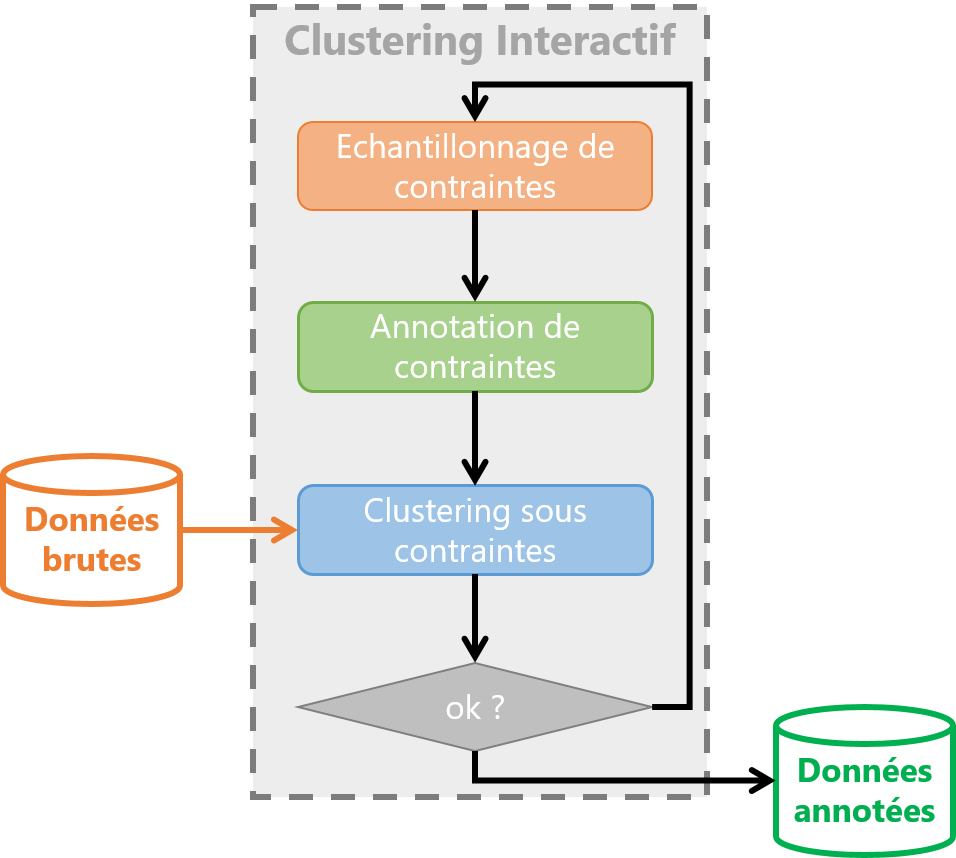
\includegraphics[width=0.85\textwidth]{figures/interactive-clustering-architecture-sequentielle}
			\caption{
				Schéma illustrant l'architecture du \texttt{Clustering Interactif}.
			}
			\label{figure:5.1-GUIDE-PRESENTATION-RAPIDE-CLUSTERING-INTERACTIF}
		\end{figure}
		
		% Figure exemple
		\begin{figure}[H]
			\centering
			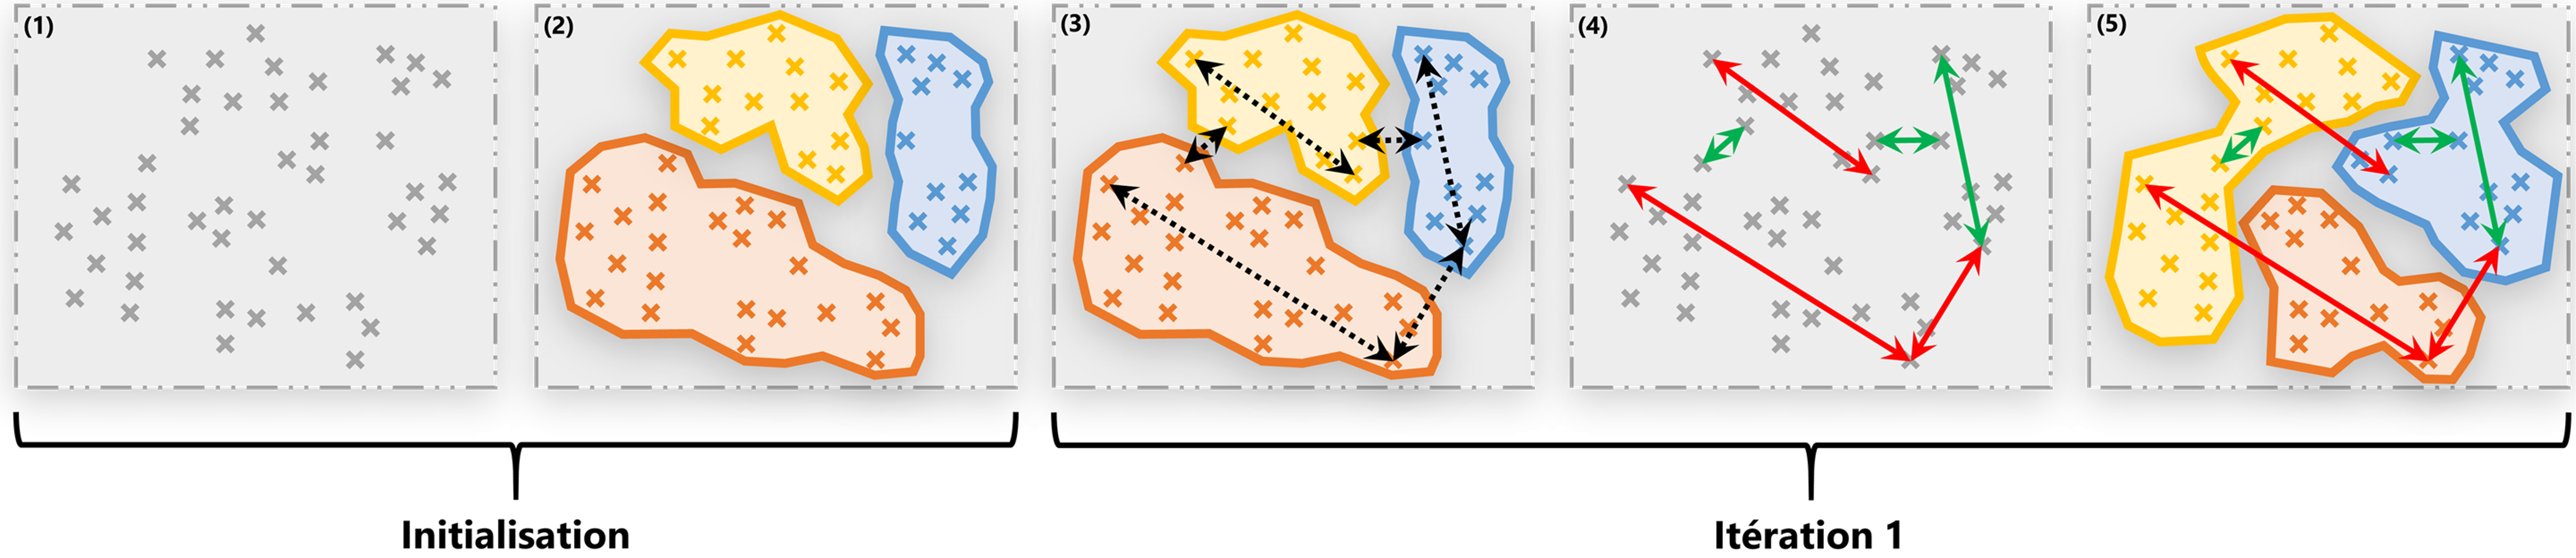
\includegraphics[width=0.85\textwidth]{figures/example-iteration-clustering-interatif}
			\caption{
				Exemple d'une itération de \texttt{Clustering Interactif}.
			}
			\label{figure:5.1-GUIDE-PRESENTATION-RAPIDE-EXEMPLE}
		\end{figure}
		
		% Références
		\begin{leftBarReminder}
			Consulter la \textsc{Section~\ref{section:3.2-DESCRIPTION-THEORIQUE}} pour plus de détails.
		\end{leftBarReminder}
	
	
	%%%%%--------------------------------------------------------------------
	%%%%% Section 5.2: Avantages et limites de la méthode.
	%%%%%--------------------------------------------------------------------
	\newpage
	\section{Avantages et limites de la méthode}
	\label{section:5.2-GUIDE-AVANTAGES-ET-LIMITES}
	
		%%% Avantages.
		Au sujet des avantages de la méthode :
		\begin{itemize}
			% Apprentissage semi-supervisé.
			\item[\textcolor{colorDarkPastelGreen}{\textcolor{colorDarkPastelGreen}{\faThumbsUp}}]
				Par conception, la méthode tire parti des avantages de l'apprentissage actif et des méthodes de regroupement semi-supervisé : \textbf{l'expert n'est plus responsable de l'ensemble du travail de labellisation} ; il intervient simplement là où il offre une valeur ajoutée (\textit{annotation des contraintes pour améliorer la pertinence de la base d'apprentissage en cours de construction}), et il délègue le reste à la machine (\textit{regroupement automatique, sélection des contraintes intéressantes à annoter, identification des incohérences}).
			% Plus de modélisation.
			\item[\textcolor{colorDarkPastelGreen}{\textcolor{colorDarkPastelGreen}{\faThumbsUp}}]
				\textbf{Il n'est plus nécessaire de définir une modélisation abstraite de la connaissance d'un expert métier pour labelliser un jeu de données} : cette modélisation est construite au cours des itérations de la méthode, à l'aide des regroupements automatiques réalisés par la machine.
			% Annotation binaire
			\item[\textcolor{colorDarkPastelGreen}{\textcolor{colorDarkPastelGreen}{\faThumbsUp}}]
				Par extension, il n'est plus nécessaire de manipuler cette modélisation abstraite pouvant contenir des dizaines d'intentions de dialogue :
				\textbf{l'expert se contente de décrire la similarité entre deux données au cours d'une annotation binaire (\texttt{MUST-LINK} ou \texttt{CANNOT-LINK})} pour corriger le résultat proposé par la machine.
			% Connaissance métier.
			\item[\textcolor{colorDarkPastelGreen}{\textcolor{colorDarkPastelGreen}{\faThumbsUp}}]
				\textbf{Cette annotation binaire se base directement sur la ressemblance entre cas d'usage métiers} : les experts intervenant dans le projet peuvent traiter les données comme ils le feraient professionnellement au quotidien, sans avoir à manipuler ou à interpréter des concepts abstraits et potentiellement non adaptés à la situation (\textit{intentions, ...}).
			% Optimisation technique et coûts compétitifs.
			\item[\textcolor{colorDarkPastelGreen}{\textcolor{colorDarkPastelGreen}{\faThumbsUp}}]
				L'implémentation de notre méthodologie d'annotation a pu être optimisée afin de converger vers une base d'apprentissage stable en un minimum de contraintes : \textbf{les coûts à engager pour cette approche semblent raisonnables et compétitifs avec l'approche d'annotation traditionnelle} (voir \textsc{Section~\ref{section:4.3.4-ETUDE-COUTS-TOTAL}}).
		\end{itemize}
	
		%%% Limites.
		Néanmoins, il faut aussi considérer quelques limites et pistes non explorées :
		\begin{itemize}
			% Sensible aux erreurs.
			\item[\textcolor{colorDarkPastelRed}{\textcolor{colorDarkPastelRed}{\faThumbsDown}}]
				Le \texttt{Clustering Interactif} possède les défauts des approches incrémentales : ainsi, \textbf{une erreur d'annotation peut rapidement se propager et pénaliser le processus}.
				Par conséquent, il est important de vérifier ses annotations (\textit{par exemple lors de session de revue avec d'autres opérateurs}), et il peut être intéressant d'introduire des contraintes redondantes afin de mieux détecter les incohérences d'annotation (voir \textsc{Section~\ref{section:4.6.2-ETUDE-ROBUSTESSE-ERREURS-ANNOTATION-ET-CORRECTION}}).
			% Sensible à la subjectivité.
			\item[\textcolor{colorDarkPastelRed}{\textcolor{colorDarkPastelRed}{\faThumbsDown}}]
				\textbf{Les différentes d'opinion entre plusieurs annotateurs concernant la caractérisation de certaines contraintes peuvent entraîner des divergences de résultat si elles ne sont pas identifiées et traitées}.
				De ce fait, il est primordial de confronter les points de vue des experts en leur faisant annoter les mêmes contraintes et en organisant des ateliers de revue pour débattre des différences d'annotation (voir \textsc{Section~\ref{section:4.6.3-ETUDE-ROBUSTESSE-SUBJECTIVITE-ANNOTATION-ET-DIVERGENCE}}).
			% Perte de visibilité dû à l'absence de modélisation.
			\item[\textcolor{colorDarkPastelRed}{\textcolor{colorDarkPastelRed}{\faThumbsDown}}]
				\textbf{La méthode peut souffrir d'un manque de visibilité et d'une sensation de perte de contrôle sur la modélisation en cours} : en effet, le processus peut être perçu comme répétitif (\textit{environ $145$ itérations à réaliser}), et le cas d'arrêt de la méthode n'est pas clairement identifiable (\textit{il est toujours possible de réaliser un itération supplémentaire pour améliorer légèrement le résultat}).
				Pour ces raisons, il est important de fournir des outils d'analyse pour tenir l'opérateur informé de son avancement et de la rentabilité de chacune de ses actions (voir \textsc{Sections}~\textsc{\ref{section:4.4-HYPOTHESE-PERTINENCE}} et~\textsc{\ref{section:4.5-HYPOTHESE-RENTABILITE}}).
		\end{itemize}
	
	
	%%%%%--------------------------------------------------------------------
	%%%%% Section 5.3: Démarche d'annotation et d'analyse de la méthode.
	%%%%%--------------------------------------------------------------------
	\newpage
	\section{Démarche d'annotation et d'analyse de la méthode}
	\label{section:5.3-GUIDE-UTILISER}
	
		%%% Annotation collaborative.
		\paragraph{\textcolor{colorSilverLakeBlue}{\faCheckSquare} Annotation collaborative.}
			
			% Constat.
			L'annotation est un acte relevant du domaine de l'interprétation et de la subjectivité.
			Par conséquent, \textbf{deux annotateurs peuvent avoir des divergences d'opinions lors de la caractérisation de la similarité entre certaines données}, ce qui peut introduire des incohérences dans le fonctionnement de notre méthode.
			Afin de limiter ces incohérences, il est nécessaire de bien définir l'objectif de l'annotation (\textit{quel est la finalité du modèle à entraîner ?}), mais aussi d'harmoniser les points de vue des différents annotateurs.
			
			% Solution.
			Au cours de l'\texttt{étude de robustesse} (voir \textsc{Section~\ref{section:4.6-HYPOTHESE-ROBUSTESSE}}), \textbf{nous conseillons d'employer au moins $3$ experts et de régulièrement (voire toujours) leur soumettre les mêmes contraintes à annoter}.
			Un tel choix semble contre-intuitif à première vue (\textit{nous triplons le coût d'embauche alors que nous pourrions tripler le nombre de contraintes annotées}), mais ce parti pris a l'avantage de contraindre les annotateurs à discuter de leurs divergences d'opinion (\textit{s'ils n'annotent pas de façon analogue, c'est qu'ils ne sont pas d'accord sur la manière de traiter les données}).
			Ainsi, même si ce choix engendre des coûts supplémentaires, il s'avère être un investissement à long terme pour garantir la qualité et la cohérence de la base d'apprentissage en cours de construction.
			
			% Notes.
			Les experts pourront annoter des contraintes différentes après plusieurs itérations de la méthode lorsque leur score d'accord inter-annotateurs sera considéré comme (très) \texttt{fort}.
		
		
		%%% Rentabilité d'une itération.
		\paragraph{\textcolor{colorSilverLakeBlue}{\faCheckSquare} Rentabilité d'une itération.}
			
			% Constat.
			Comme notre méthodologie est itérative, il faut être capable de définir un cas d'arrêt (\textit{annoter toutes les contraintes possibles étant trop ambitieux}).
			
			% Solution.
			Au cours de l'\texttt{étude de rentabilité} (voir \textsc{Section~\ref{section:4.5-HYPOTHESE-RENTABILITE}}), nous avons mis en évidence l'intérêt d'\textbf{analyser l'évolution de la différence de résultats de \textit{clustering} entre deux itérations consécutives afin de quantifier l'intérêt d'une itération supplémentaire}.
			En effet, si le nouveau \textit{clustering} reste fortement similaire au \textit{clustering} précédent, malgré l'ajout de contraintes supplémentaires, nous pouvons en déduire que la méthode d'annotation stagne.
			Il peut alors être intéressant d'envisager de stopper les itérations de la méthode, d'évaluer la pertinence métier du \textit{clustering} actuel, et de corriger manuellement les reliquats.
			
			% Mise en oeuvre.
			Pour estimer cette différence entre deux \textit{clustering} consécutifs, nous utilisons le score de \texttt{v-measure} (voir \textsc{Annexe~\ref{annex:D-ANNEXE-EVALUATION-CLUSTERING}}).
		
		
		%%% Pertinence d'un résultat.
		\paragraph{\textcolor{colorSilverLakeBlue}{\faCheckSquare} Pertinence d'un résultat.}
			
			% Constat.
			L'analyse d'un résultat de \textit{clustering} n'est pas une tâche aisée, et elle peut vite devenir fastidieuse si elle doit être faite à chaque itération de notre méthode.
			
			% Solution.
			Au cours de l'\texttt{étude de pertinence} (voir \textsc{Section~\ref{section:4.4-HYPOTHESE-PERTINENCE}}), nous avons proposé deux solutions prometteuses pour assister l'expert dans cette évaluation :
			\begin{itemize}
				% FMC.
				\item Une \textbf{analyse des patterns linguistiques caractéristiques de chaque \textit{cluster} en utilisant la \texttt{FMC}} (voir \textsc{Annexe~\ref{annex:C.3-DESCRIPTION-IMPLEMENTATION-FEATURES-MAXIMIZATION-METRIC}}) :
				un \textit{cluster} peut ainsi être identifié comme pertinent s'il possède un vocabulaire caractéristique cohérent du point de vue de l'expert.
				Il est aussi possible de se servir de cette analyse pour identifier dans chaque texte les mots caractéristiques d'un ou plusieurs \textit{clusters}.
				% LLM.
				\item Un \textbf{résumé thématique des \textit{clusters} par un large modèle de langage (\texttt{LLM})} :
				cette approche permet d'estimer efficacement la cohérence d'un \textit{cluster} à l'aide d'une courte description en langage naturel.
				Il faut toutefois être vigilant aux hallucinations du \texttt{LLM}.
			\end{itemize}
			
			% Constat.
			Note : \textbf{Une correction manuelle est parfois nécessaire} pour valider un \textit{cluster}.
	
	
	%%%%%--------------------------------------------------------------------
	%%%%% Section 5.4: Implémentation et paramétrages de la méthode.
	%%%%%--------------------------------------------------------------------
	\newpage
	\section{Implémentation et paramétrages de la méthode}
		\label{section:5.4-GUIDE-PARAMETRAGES}
		
		%%% Références aux implémentations.
		\paragraph{\textcolor{colorSilverLakeBlue}{\faCheckSquare} Développements logiciels.}
		
			% Références.
			Pendant ce doctorat, nous avons implémenté plusieurs algorithmes de \textit{clustering} et d'échantillonnage (\textit{disponibles dans \cite{schild:2022:cognitivefactory-interactiveclustering}}) et nous avons intégré notre méthodologie d'annotation dans une application web (\textit{accessible dans \cite{schild-etal:2022:cognitivefactory-interactiveclusteringgui}}).
			Ces développements logiciels sont décrits en \textsc{Annexe~\ref{annex:C-ANNEXE-IMPLEMENTATIONS}}.
		
		%%% Paramétrage optimal.
		\paragraph{\textcolor{colorSilverLakeBlue}{\faCheckSquare} Choix des paramétrages.}
		
			% Description.
			Au cours de nos études (voir \textsc{Chapitre~\ref{chapter:4-ETUDES}}), nous avons mis en avant un \textbf{paramétrage favori} de notre méthode.
			Ce paramétrage, basé sur un compromis entre un maximum d'efficience et un minimum de coûts, est composé des algorithmes suivants :
			
			% Liste paramètres.
			\begin{itemize}
				\item \texttt{prep.simple}: les \textbf{prétraitements} \textbf{simples} supprimant les minuscules, les ponctuations, les accents et les espaces blancs ;
				\item \texttt{vect.tfidf}: la \textbf{vectorisation} utilisant une représentation statistique du vocabulaire à l'aide d'un \texttt{TF-IDF} (\cite{ramos:2003:using-tfidf-determine}) ;
				\item \texttt{clust.kmeans.cop}: le \textbf{\textit{clustering} sous contraintes} utilisant l'algorithme \textbf{\texttt{COP-KMeans}} (\cite{wagstaff-etal:2001:constrained-kmeans-clustering}) ;
				\item \texttt{samp.closest.diff}: l'\textbf{échantillonnage de contraintes} concernant des données issues de \textbf{\textit{clusters} différents} et étant \textbf{les plus proches} les unes des autres.
			\end{itemize}
		
			% Temps de calcul.
			Une approximation du temps de calcul d'une itération de \texttt{Clustering Interactif} utilisant ce paramétrage favori est estimée avec l'\textsc{Équation~\ref{equation:5.4-GUIDE-PARAMETRAGES-TEMPS-CALCUL}}.
			
			% Equation.
			\begin{equation}
				\label{equation:5.4-GUIDE-PARAMETRAGES-TEMPS-CALCUL}
				\texttt{computation\_time}~[s]~\propto~0.17 \cdot \texttt{dataset\_size}
			\end{equation}
		
		
		%%% Parallélisation.
		\paragraph{\textcolor{colorSilverLakeBlue}{\faCheckSquare} Choix d'architecture}
		
			% Description.
			Au lieu de réaliser les étapes du \texttt{Clustering Interactif} de manière séquentielle, il peut être intéressant d'\textbf{implémenter une architecture parallèle} de notre méthode (voir \textsc{Figure~\ref{figure:5.4-GUIDE-PARAMETRAGES-ARCHITECTURE-PARALLELE}}).
			Une telle approche consiste à faire coïncider les temps de calcul et d'annotation dans le but de diminuer les temps d'attente : une approximation du nombre de contraintes déterminant l'équivalence de ces durées est estimée avec l'\textsc{Équation~\ref{equation:5.4-GUIDE-PARAMETRAGES-ANNOTATION-BATCH}}.
			
			% Equation.
			\begin{equation}
				\label{equation:5.4-GUIDE-PARAMETRAGES-ANNOTATION-BATCH}
				\texttt{annotation\_batch\_size}~[\#]~\propto~0.0218 \cdot \texttt{dataset\_size}
			\end{equation}
			
			% Figure.
			\begin{figure}[H]
				\centering
				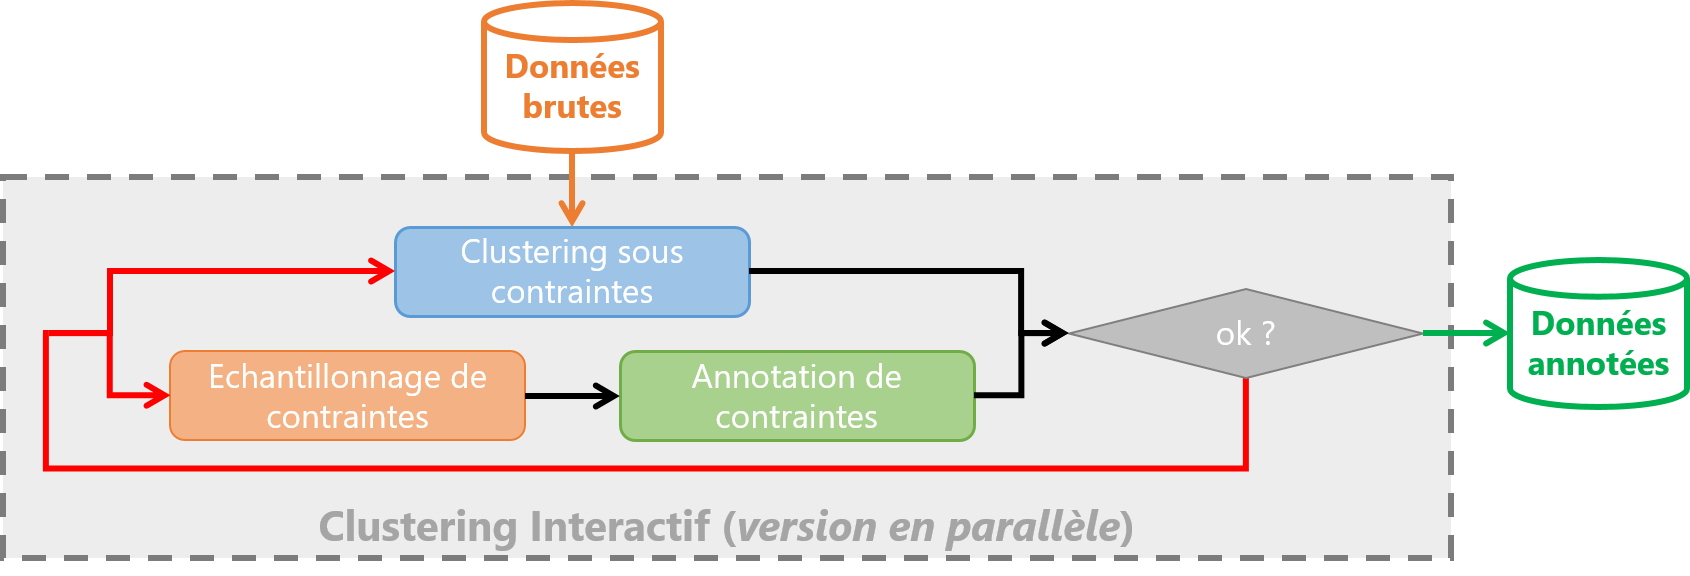
\includegraphics[width=0.85\textwidth]{figures/interactive-clustering-architecture-parallele}
				\caption{
					Schéma illustrant l'architecture du \texttt{Clustering Interactif} en mode parallèle.
				}
				\label{figure:5.4-GUIDE-PARAMETRAGES-ARCHITECTURE-PARALLELE}
			\end{figure}
	
	
	%%%%%--------------------------------------------------------------------
	%%%%% Section 5.5: Estimation des coûts de la méthode.
	%%%%%--------------------------------------------------------------------
	\newpage
	\section{Estimation des coûts de la méthode}
	\label{section:5.5-GUIDE-COUTS}
	
		% Introduction.
		Dans nos études, et principalement au cours de la \textsc{Section~\ref{section:4.3-HYPOTHESE-COUTS}}, nous avons pu estimer un ensemble de coûts théoriques (temporels et humains) estimés grâce aux jeux de données \texttt{Bank Cards} (\cite{schild:2022:french-trainset-chatbots}) et \texttt{MLSUM} (\cite{schild-adler:2023:subset-mlsum-multilingual}).
		
		
		%%% Vitesse d'annotation.
		\paragraph{\textcolor{colorSilverLakeBlue}{\faCheckSquare} Vitesse d'annotation}
			
			% Description.
			À l'aide d'une expérience en situation réelle, nous avons estimé qu'\textbf{il faut environ $7.8$ secondes pour caractériser une contrainte}.
			Nous avons montré que ce temps est inférieur à celui d'une annotation d'étiquettes faisant intervenir une modélisation ;
			l'annotation de contraintes est donc \textit{a priori} moins complexe et plus rapide.
		
		
		%%% Nombre de contraintes.
		\paragraph{\textcolor{colorSilverLakeBlue}{\faCheckSquare} Nombre de contraintes nécessaires}
		
			% Description.
			À l'aide d'une simulation, nous avons estimé qu'\textbf{il faut environ $3.15$ contraintes par donnée pour obtenir une base d'apprentissage stable} (\textit{bien entendu, cette estimation doit varier grandement en fonction la complexité des données et la finalité du modèle à entraîner}).
			Nous rappelons qu'un expert métier devra confirmer la pertinence du \textit{clustering} avant d'arrêter la méthode.
			Il est toutefois intéressant de noter que cette estimation du nombre de contraintes nécessaires est linéaire alors que le nombre de contraintes possibles augmente de manière quadratique avec le nombre de données.
		
		
		%%% Temps total.
		\paragraph{\textcolor{colorSilverLakeBlue}{\faCheckSquare} Temps total théorique}
		
			% Description.
			En utilisant une architecture parallèle, nous estimons qu'\textbf{il faut environ $24.6$ secondes par donnée pour obtenir une base d'apprentissage stable}.
			Nous pouvons aussi noter qu'une telle approche propose un nombre constant de $144.5$ itérations pour annoter le nombre de contraintes requis afin d'obtenir une base d'apprentissage stable.
			
			% Comparaison avec une approche classique.
			Une telle estimation semble compétitive avec une annotation d'étiquettes faisant intervenir une modélisation : en effet, le temps d'annotation est légèrement plus long (\textit{à cause du nombre de contraintes à traiter}), mais nous économisons le temps nécessaire à la formation des experts ainsi qu'aux nombreuses révisions de modélisation en intentions intentions.
		
		
		%%% Robustesse et nombre d'annotateurs.
		\paragraph{\textcolor{colorSilverLakeBlue}{\faCheckSquare} Coûts d'analyse et de robustesse}
			
			% Attention.
			Il est à noter que \textbf{de nombreux coûts n'ont pas pu être estimés} (\textit{ces derniers étaient impossibles à simuler ou à reproduire}) :
			\begin{itemize}
				% Temps d'analyse.
				\item Le \textbf{temps nécessaire à l'analyse de la pertinence et de la rentabilité}
				(\textit{les gains de temps liés à nos approches pour assister ces étapes n'ont pas pu être estimés}).
				% Trois annotateurs.
				\item Nous avons conseillé d'\textbf{employer plusieurs experts annotant les mêmes données} : ce choix augmente le coût d'embauche, mais cet investissement garantit la cohérence des annotations et évite la conception d'une modélisation abstraite des données.
				% Temps de revue et de débats.
				\item Le \textbf{temps nécessaire aux revues d'annotations et aux débats d'opinion entre annotateurs} : de tels coûts existent aussi pour les approches traditionnelles, cependant les échanges sont ici davantage concrets car ils se basent sur les similarités de cas d'usage.
			\end{itemize}
			
			% Conseils.
			Par conséquent, \textbf{nous conseillons d'utiliser les estimations ci-dessous avec une marge d'erreur proportionnelle à la quantité et à la complexité des données à annoter}.
			
		% Equation.
		\begin{equation}
			\label{equation:5.5-GUIDE-COUTS}
			\begin{cases}
				\texttt{annotation\_time}~[s] &
					~\propto~7.8 \cdot \texttt{batch\_size} \\
				\texttt{constraints\_needed}~[\#] &
					~\propto~3.15 \cdot \texttt{dataset\_size} \\
				% Total time.
				\texttt{total\_time}~[s] &
					~\propto~24.6 \cdot \texttt{dataset\_size} \\
				% Iterations number.
				\texttt{iterations\_needed}~[\#] &
					~\propto~144.5
			\end{cases}
		\end{equation}
	
	
	%%%%%--------------------------------------------------------------------
	%%%%% Section 5.6: Conseils pour rédiger le guide d'annotation.
	%%%%%--------------------------------------------------------------------
	\newpage
	\section{Conseils pour rédiger le guide d'annotation}
		\label{section:5.6-GUIDE-REDIGER}
		
		% Introduction.
		Nous terminons ce chapitre de bilan en listant quelques conseils pour bien cadrer un projet de conception de base d'apprentissage utilisant notre méthode d'annotation.
		\begin{leftBarInformation}
			Nous nous référons aux $7$ maximes proposées par \cite{leech:1993:corpus-annotation-schemes} (et détaillées par \cite{fort:2022:manual-annotation-what}) que nous allons adapter pour le cas d'annotation de contraintes.
		\end{leftBarInformation}
		
		% Conseils basés sur les 7 maximes de Leech.
		\begin{enumerate}
			%  1. It should always be possible to come back to initial data.
			\item \textbf{La donnée initiale doit toujours pouvoir être accessible} \footnote{
				Maxime $1$ : \textguillemets{\textit{It should always be possible to come back to initial data.}}
			} :
			en effet, il faut faire attention aux étapes de prétraitements et de nettoyage qui peuvent effacer des informations potentiellement importantes pour l'analyse.
			% 2. Annotations should be extractable from the text.
			\item \textbf{L'annotation d'une contrainte doit se baser sur des similarités ou des différences observables} \footnote{
				Maxime $2$ : \textguillemets{\textit{Annotations should be extractable from the text.}}
			} :
			en effet, si aucun indice ne permet de faire un choix objectif, il est préférable de s'abstenir (\textit{voire de supprimer la donnée si elle est trop ambiguë}).
			% 3. The annotation procedure should be documented.
			\item \textbf{Il faut documenter l'objectif de l'annotation de contraintes et expliciter clairement sur quels critères elle se base} \footnote{
				Maxime $3$ : \textguillemets{\textit{The annotation procedure should be documented.}}
			} :
			d'une part, il est important de décrire sur quoi caractériser la similarité entre les données (\textit{sur l'action ? sur l'objet de l'action ? sur le sentiment associé ? ...}) ;
			d'autre part, cette documentation doit être complétée au fur et à mesure des revues d'annotation et des résolutions d'incohérences dans la base de contraintes (\textit{dans telle situation, la similarité sera caractérisée de telle manière}).
			% 4. Mention should be made of the annotator(s) and the way annotation was made.
			\item \textbf{Il est important de  décrire les opérateurs réalisant les annotations} \footnote{
				Maxime $4$ : \textguillemets{\textit{Mention should be made of the annotator(s) and the way annotation was made.}}
			} :
			leur nombre, leur expertise du sujet traité, leur formation à la tâche d'annotation, les outils d'assistance à leur disposition, les biais potentiels au cours de l'annotation, \textit{etc}.
			% 5. Annotation is an act of interpretation (cannot be infallible).
			\item \textbf{L'annotation est toujours une action d'interprétation} \footnote{
				Maxime $5$ : \textguillemets{\textit{Annotation is an act of interpretation (cannot be infallible).}}
			} : elle est donc forcément subjective et entraînera des différences d'annotations qui devront être discutées lors de revues entre opérateurs.
			% 6. Annotation schemas should be as independent as possible on formalisms.
			\item \textbf{Il est nécessaire d'être rigoureux dans l'annotation de contraintes pour ne pas introduire des incohérences ou produire des regroupements imprévus} \footnote{
				Maxime $6$ : \textguillemets{\textit{Annotation schemas should be as independent as possible on formalisms.}}
			} :
			dans le doute, il est préférable de s'abstenir de caractériser une contrainte et de laisser la machine décider du regroupement le plus adéquat au regard du reste du jeu de données.
			% 7. No annotation schema should consider itself a standard (it possibly becomes one).
			\item \textbf{À cause de la subjectivité de la tâche, plusieurs visions peuvent être envisagées pour annoter la similarité} \footnote{
				Maxime $7$ : \textguillemets{\textit{No annotation schema should consider itself a standard (it possibly becomes one).}}
			} :
			l'important est de pouvoir en discuter (\textit{au moins à trois personnes}), de choisir le point de vue qui semble le plus adapté au regard de la finalité du modèle à entraîner, et de s'y tenir pour limiter les incohérences.
		\end{enumerate}